\section{Systems Analysis}
\label{sec:systems_analysis}

The algorithm is derived from the flight-system constraints.
Rather than solve an adaptive stochastic scheduling problem with continuous lookahead times, continuous pointing angles, unknown cloud states, and a combinatorial imaging schedule, we first use spacecraft geometry and agility limits to collapse dynamic tasking into local decisions made in schedule gaps.
For each gap, the spacecraft asks whether one lookahead maneuver is physically meaningful and, if so, what pitch angles are feasible.
The lookahead decision method in the next section then estimates whether any feasible maneuver has positive schedule-level value.

\subsection{Dynamic Tasking Formulation}
\label{sec:dt_formulation}

Conventional scheduling treats access utilities $u_i$ as known. In practice they are modulated by cloud state:
\begin{equation}
u_i = c_i \cdot \mathbf{1}_{\{\text{clear}(r_i, t_i)\}},
\end{equation}
where $c_i$ is intrinsic value and $\mathbf{1}_{\{\cdot\}}$ indicates cloud-free conditions.
We focus on the \emph{unit-utility} case ($c_i = 1$), isolating when to look from task-value heterogeneity; the heavy-tailed utility regime is treated in~\cite{kacker_spacecraft_2025}.
Cloud state is unknown when the ground schedule is produced, but can be revealed by a \emph{lookahead observation} that points a secondary wide-field instrument toward upcoming targets and triggers schedule repair with updated utilities.

A lookahead therefore has two coupled effects: \emph{advantage} from revealing clear accesses that may be inserted into the repaired schedule, and \emph{opportunity cost} from consuming slew time that could otherwise be used for imaging.
The systems problem is to decide which lookahead actions are physically meaningful; the algorithmic problem is to estimate whether their expected advantage exceeds their cost using only onboard information.

This paper analyzes the body-fixed onboard-lookahead case because it is the most tightly coupled to spacecraft agility: the same bus that images targets must also slew to acquire information about them.
Other dynamic-tasking architectures, including leader-follower constellations, sensor webs, and real-time meteorological-data feeds, shift this trade to communication latency, sensor cadence, and data-fusion assumptions~\citep{chien_autonomous_2005, chien_automated_2020, chien_using_2019, kacker_leveraging_2025, mahonchak_goes-r_nodate}.
The body-fixed case therefore provides a constrained reference problem in which field of view, horizon lead time, and slew time directly determine the feasible onboard decision space.

\subsection{Baseline Scheduling Model}
\label{sec:scheduling}

An Earth-observing satellite receives imaging requests $\mathcal{R}$ and, given an orbit, converts each request into a set of \emph{accesses} $\mathcal{A}$.
Operational requests may be point, strip, or area collects; for this analysis they are represented as point access opportunities, following the standard EO scheduling pipeline that tessellates or decomposes requests before access generation~\citep{eddy_task_2021, xu_multi-satellite_2020}.
Each access $a_i = (r_i, t_i, \theta_i)$ records the request, overpass time, and off-nadir roll angle, following~\cite{eddy_task_2021}.
The scheduling problem is to select a subset $\boldsymbol{\sigma} \subseteq \mathcal{A}$ maximizing total utility subject to agility constraints:
\begin{equation}
\max_{\boldsymbol{\sigma}} \sum_{a_i \in \boldsymbol{\sigma}} u_i, \quad
\text{s.t.} \quad t_j - t_i \geq t_{\mathrm{slew}}(\theta_j - \theta_i) \;\;\forall\; a_i, a_j \in \boldsymbol{\sigma},\; t_j > t_i,
\label{eq:scheduling}
\end{equation}
where the slew time follows a bang-bang agility model $t_{\mathrm{slew}}(\Delta\theta) = t_s + \beta\sqrt{|\Delta\theta|}$, with settling time $t_s$ and rate parameter $\beta$.
We solve~\eqref{eq:scheduling} via mixed-integer linear programming (MILP), with an additional repetition constraint preventing multiple accesses of the same request.

\subsection{Lookahead Geometry and Agility Constraints}
\label{sec:lookahead_design}

We consider a body-fixed secondary instrument pointed ahead of nadir toward the horizon.
The systems design determines the algorithmic action space: a lookahead action is feasible only if its field of view covers useful future accesses and the spacecraft can complete the maneuver before the next scheduled image.
Two assumptions fix the geometry: the spacecraft's neutral position after imaging is nadir-pointed, and the lookahead field of view has its bottom edge at nadir (so boresight pitch equals half the vertical FoV).
This is intentionally the constrained case: electronically steerable lookahead sensors, fold mirrors, and radar-based sensing can partially decouple observation from bus agility~\citep{imasu_greenhouse_2023, bosch-lluis_smart_2022}, but a body-fixed payload makes the agility and field-of-view requirements explicit.

\paragraph{Spherical geometry.}
Let $a = R_E + h$ be the orbital radius and $n = \sqrt{\mu/a^3}$ the mean motion.
A point at the horizon reaches nadir after
\begin{equation}
t_{\mathrm{horizon}} = \frac{1}{n} \arccos\!\left(\frac{R_E}{a}\right),
\label{eq:horizon}
\end{equation}
giving $t_{\mathrm{horizon}} \approx \SI{305}{\second}$ at $h = \SI{400}{\kilo\metre}$ and bounding the maximum observation lead time.
In \figref{fig:lookahead_geometry}, a ray from spacecraft $S$ pitched ahead by angle $\alpha$ intersects Earth at $P$ and subtends the Earth-centered angle $\angle NOP$:
\begin{equation}
\psi(\alpha) = \arccos\!\left(\frac{a\sin^2\alpha + \cos\alpha\,\sqrt{R_E^2 - a^2 \sin^2\alpha}}{R_E}\right)
\label{eq:dtrack}
\end{equation}
from nadir and reaches nadir after $t_{\mathrm{point}}(\alpha) = \psi(\alpha)/n$.
The same ray intersection also has a local coordinate in the plane through $N$ tangent to the local horizontal:
\begin{equation}
\rho(\alpha) =
\sin\alpha \left[a\cos\alpha -
\sqrt{R_E^2 - a^2 \sin^2\alpha}\right].
\label{eq:ground_offset}
\end{equation}
In the diagram, $\psi(\alpha)$ is the central angle $\angle NOP$.
The companion flat-plane quantity $\rho(\alpha)$ is the local-horizontal projection of $NP$: the signed distance, in the plane tangent to Earth at $N$, from $N$ to the projection of $P$ along the local vertical direction $ON$.
It is therefore not the curved ground distance along the surface, but the coordinate used to place ray hits in the local detector geometry below.
The same spherical setup is used below for both lookahead timing and field-of-view sizing.

\begin{figure}[htb]
    \centering
    \begin{subfigure}[b]{0.36\textwidth}
        \centering
        \raisebox{1.2em}{%
        \resizebox{\linewidth}{!}{%
        \begin{tikzpicture}[
            dot/.style = {circle, fill=black, inner sep=2pt},
            lbl/.style = {label distance=-0.7mm},
            >=latex]
            \def\r{4}
            \def\dphi{20}
            \coordinate (O) at (0,0);
            \coordinate (S) at (0,1.5*\r);
            \coordinate (P) at ({\r*cos 75},{\r*sin 75});
            \coordinate (H) at ({\r*sqrt(5)/3},{2*\r/3});
            \coordinate (N) at (0,\r);
            \draw[thick,dashed] ({\r*cos 100},{\r*sin 100})
                arc[start angle=100,end angle=100+\dphi,radius=\r];
            \draw[thick] ({\r*cos 100},{\r*sin 100})
                arc[start angle=100,end angle=20,radius=\r];
            \draw[thick,dashed] ({\r*cos 20},{\r*sin 20})
                arc[start angle=20,end angle=20-\dphi,radius=\r];
            \draw[thick] (S) -- (N) node[midway,xshift=-3mm] {$h$};
            \draw[thick] (N) -- (O) node[midway,xshift=-3mm] {$R_E$};
            \draw[thick] (O) -- (H) node[midway,sloped,above=-0.7mm] {$R_E$};
            \draw[thick] (H) -- (S);
            \draw[thick] (O) -- (P) -- (S);
            \pic [draw, angle radius=4mm] {right angle = O--H--S};
            \pic [draw, angle radius=6mm, "$\alpha$", angle eccentricity=1.35] {angle = N--S--P};
            \node[dot,label={[lbl]below right:$O$}] at (O) {};
            \node[dot,label={[lbl]above right:$S$}] at (S) {};
            \node[dot,label={[lbl, xshift=-1mm]below right:$P$}] at (P) {};
            \node[dot,label={[lbl]above right:$H$}] at (H) {};
            \node[dot,label={[lbl]below right:$N$}] at (N) {};
        \end{tikzpicture}%
        }}
        \caption{Spherical geometry.}
        \label{fig:lookahead_geometry}
    \end{subfigure}
    \hfill
    \begin{subfigure}[b]{0.6\textwidth}
        \centering
        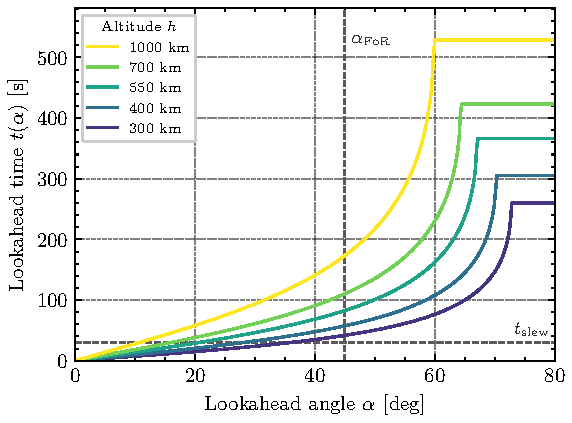
\includegraphics[width=\textwidth]{figures/lookahead_time_constraints.pdf}
        \caption{Lookahead time over altitude.}
        \label{fig:lookahead_time_altitudes}
    \end{subfigure}
    \caption{Lookahead geometry and timing. \textbf{(a)} Spacecraft at $S$, nadir projection $N$, horizon tangent $H$, and target $P$ at pitch angle $\alpha$. The central angle $\angle NOP$ is $\psi(\alpha)$, while the local-horizontal projection of $NP$ is $\rho(\alpha)$. \textbf{(b)} Lookahead time $t(\alpha)$ for representative LEO altitudes. A lookahead is actionable where $t(\alpha) \geq t_{\mathrm{slew}}$ and $\alpha \leq \alpha_{\mathrm{FoR}}$.}
    \label{fig:lookahead_time_constraints}
\end{figure}

\paragraph{Vertical FoV.}
Three timing constraints act on the vertical FoV:
\begin{itemize}
    \item \textbf{Slew time:} the instrument must see ahead far enough that every task within the off-nadir field of regard is still reachable after a full cross-track slew.
    \item \textbf{Pitching field of regard:} in the worst case---pitched fully backward within the field of regard---the instrument must still observe beyond nadir.
    \item \textbf{Settling time:} even when a task is visible, the maneuver plus settling may leave no feasible action, defining regions where a lookahead is \emph{never} net-positive.
\end{itemize}
\figref{fig:lookahead_time_constraints} plots $t(\alpha)$ across LEO altitudes. A lookahead is actionable only where $t(\alpha) \geq t_{\mathrm{slew}}$ and $\alpha \leq \alpha_{\mathrm{FoR}}$.

\paragraph{Horizontal FoV.}
Horizontal constraints depend on the primary imager field of regard $\theta_{\mathrm{FoR}}$ and take two forms:
\begin{itemize}
    \item \textbf{Nadir FoR:} both edges of the field of regard must lie within the sensor FoV when the spacecraft is at nadir.
    \item \textbf{Rolled FoR:} the lookahead footprint must reach the field-of-regard edges when the spacecraft is rolled to the maximum off-nadir angle to acquire an image.
\end{itemize}
Let $\Theta_h$ denote the full horizontal FoV and let $\beta=\Theta_v/2$.
The horizontal calculation reuses the same plane tangent at $N$ in \figref{fig:lookahead_geometry}, but now with one local-horizontal coordinate $x$ forward along track and one coordinate $y$ cross track.
The coordinate $x$ is the same type of local-horizontal projection as $\rho(\alpha)$ in the spherical-geometry paragraph.
A primary-imager FoR edge has cross-track projection $\rho_F=\rho(\theta_{\mathrm{FoR}})$, so points on the two FoR edges have local-horizontal coordinates $(x,\pm\rho_F)$ before detector projection.
\figref{fig:tangent_plane_frame} summarizes this local frame.

\begin{figure}[htbp]
    \centering
    \begin{tikzpicture}[
        >=Latex,
        x=1cm,
        y=1cm,
        point/.style={circle, fill=black, inner sep=1.5pt},
        edge/.style={thick, gray!65},
        guide/.style={densely dotted, gray!70},
        lbl/.style={font=\small}
    ]
        \coordinate (N) at (0,0);
        \coordinate (Pproj) at (2.15,0);
        \coordinate (Q) at (3.6,1.05);

        \draw[->, thick] (-0.35,0) -- (4.75,0) node[right,lbl] {$x$ forward};
        \draw[->, thick] (0,-1.55) -- (0,1.65) node[above,lbl] {$y$ cross track};

        \draw[edge] (-0.15,1.05) -- (4.25,1.05) node[right,lbl, gray!70] {$y=+\rho_F$};
        \draw[edge] (-0.15,-1.05) -- (4.25,-1.05) node[right,lbl, gray!70] {$y=-\rho_F$};
        \node[lbl, gray!70, anchor=west] at (0.7,1.42) {FoR-edge slice};

        \node[point,label={[lbl]below left:$N$}] at (N) {};
        \node[point] at (Pproj) {};
        \node[lbl, align=center] at (2.15,0.34) {vertical\\projection of $P$};
        \node[point] at (Q) {};
        \node[lbl, anchor=south, fill=white, inner sep=1pt] at (Q) {$(x,\rho_F)$};

        \draw[guide] (Pproj) -- ++(0,1.05);
        \draw[guide] (Q) -- ++(0,-1.05);
        \draw[<->] (0,-0.72) -- node[fill=white, inner sep=1pt, lbl] {$\rho(\alpha)$} (2.15,-0.72);
        \draw[<->] (-0.45,0) -- node[fill=white, inner sep=1pt, lbl] {$\rho_F$} (-0.45,1.05);
        \draw[<->] (0,0.74) -- node[fill=white, inner sep=1pt, lbl] {$x$} (3.6,0.74);

        \node[lbl, align=center, text width=3.6cm] at (2.15,-1.35)
            {plane tangent to Earth at $N$};
    \end{tikzpicture}
    \caption{Local tangent-plane frame used for horizontal-FoV sizing. The spherical diagram defines $N$ and $P$; here $P$ is projected onto the plane tangent at $N$ along the local vertical direction $ON$. The primary-imager FoR edges become the two lines $y=\pm\rho_F$, and fixing one edge gives the Earth slice used to define $R_F$ and $z(x)$.}
    \label{fig:tangent_plane_frame}
\end{figure}

The corresponding fixed-FoR-edge Earth slice has radius and nadir-axis depth
\begin{equation}
R_F=\sqrt{R_E^2-\rho_F^2},\qquad
z(x)=a-\sqrt{R_F^2-x^2}.
\label{eq:for_edge_slice}
\end{equation}
The subscript $F$ denotes this fixed FoR-edge slice.
Here $z(x)$ is the component of the vector from $S$ to the surface point along the spacecraft-nadir direction $SN$.
The analogue of horizon point $H$ on one of these fixed-FoR-edge slices is the limb point on that FoR edge: the point where the ray from $S$ is tangent to Earth.
Its forward coordinate is
\begin{equation}
x_{\mathrm{limb}}=\sqrt{R_E^2\left(1-\left[\frac{R_E}{a}\right]^2\right)-\rho_F^2}.
\label{eq:for_horizon_cap}
\end{equation}
Thus $x_{\mathrm{limb}}$ is not a field-of-view angle: detector contacts beyond it are physically beyond Earth and are replaced by the limb point on the same FoR edge.
Once $\Theta_v$ is chosen, the forward edge of the lookahead lies at off-nadir angle $\Theta_v$ because the lower edge is fixed at nadir.
Both horizontal constraints are obtained by projecting the two FoR edges into the same rectilinear detector plane; Appendix~\ref{sec:appendix_fov_projection} gives the shared map.
The useful closed forms below are the nadir and rolled specializations of that map.

For the nadir attitude, $\varphi=0$ and the two FoR edges are symmetric.
The limiting forward coordinate is the first contact between the upper detector edge and the FoR edge, unless that contact lies past the limb:
\begin{equation}
\begin{aligned}
\Theta_v^{\mathrm{limb}}
&=\arcsin\!\left(\frac{R_F}{a}\right),\\
x_{\mathrm{edge}}
&=\sin\Theta_v
\left[
a\cos\Theta_v
-\sqrt{R_F^2-a^2\sin^2\Theta_v}
\right],\\
x_{\mathrm{nadir}}
&=
\begin{cases}
x_{\mathrm{edge}}, & \Theta_v\leq\Theta_v^{\mathrm{limb}},\\
x_{\mathrm{limb}}, & \Theta_v>\Theta_v^{\mathrm{limb}},
\end{cases}
\end{aligned}
\label{eq:nadir_closed_form_terms}
\end{equation}
The nadir-FoR horizontal requirement is then
\begin{equation}
\Theta_h^{\mathrm{nadir}} \geq
2\arctan\!\left(
\frac{\rho_F}{x_{\mathrm{nadir}}\sin\beta+z(x_{\mathrm{nadir}})\cos\beta}
\right).
\label{eq:horizontal_fov_requirement}
\end{equation}

For the rolled-body attitude, set $\varphi$ to the maximum body roll; in the design maps below, $\varphi=\theta_{\mathrm{FoR}}$.
This pins the same-side FoR point to the lower detector center, so the opposite FoR edge sets the horizontal width.
The rolled upper-edge contact needs only the detector-edge slope and the rolled range offset
\begin{equation}
Q=\cot(2\beta),\qquad
K_-=a\cos\varphi-\rho_F\sin\varphi.
\end{equation}
Here $Q$ comes from the upper detector edge because the lower edge is fixed at nadir, while $K_-$ collects the body-roll projection of the opposite FoR edge.
The front-facing upper-edge contact $x_{\mathrm{upper}}$ is the retained root of
\begin{equation}
x_{\mathrm{upper}}\in
\left\{
\frac{K_-Q \pm
\sqrt{K_-^2Q^2-\left(\cos^2\varphi+Q^2\right)
\left(K_-^2-\cos^2\varphi\,R_F^2\right)}}
{\cos^2\varphi+Q^2}
\right\},
\label{eq:rolled_upper_contact_closed_form}
\end{equation}
where $x_{\mathrm{upper}}$ denotes the physically retained root on the opposite FoR edge; if both signs are admissible, use the one with smaller horizontal look angle.
The limiting opposite-edge contact is
\begin{equation}
x_{\mathrm{roll}} =
\begin{cases}
x_{\mathrm{limb}}, & \text{the limb point is inside the detector band},\\
x_{\mathrm{upper}}, & \text{otherwise, if an upper-edge contact exists},\\
\text{infeasible}, & \text{otherwise}.
\end{cases}
\label{eq:rolled_opposite_contact}
\end{equation}
The rolled horizontal-FoV requirement is then
\begin{equation}
\Theta_h^{\mathrm{roll}}
\geq
2\left|
\operatorname{atan2}\!\left(
-\rho_F\cos\varphi-z(x_{\mathrm{roll}})\sin\varphi,\,
x_{\mathrm{roll}}\sin\beta+
\left[z(x_{\mathrm{roll}})\cos\varphi-\rho_F\sin\varphi\right]\cos\beta
\right)
\right|.
\label{eq:rolled_body_horizontal_requirement}
\end{equation}
Appendix~\ref{sec:appendix_nadir_fov} derives the nadir contact, and Appendix~\ref{sec:appendix_rolled_fov} derives~\eqref{eq:rolled_upper_contact_closed_form} and gives the exact admissibility tests used for implementation.
When $\theta_{\mathrm{FoR}}\approx\ang{45}$, the opposite FoR edge lies near the front-facing horizon of the rolled camera at the lower edge.
For small vertical FoV it may never enter the rectangular focal-plane band while still in front of the detector, producing a genuinely infeasible body-fixed view.
As $\Theta_v$ increases, the admissible band reaches farther forward on that edge and finite horizontal-FoV contacts reappear.
\figref{fig:horizontal_fov_design_map} compares the nadir and rolled-body constraints.
For $\theta_{\mathrm{FoR}}\gtrsim\ang{45}$, the infeasible region persists until the vertical band reaches sufficiently far forward on the opposite FoR edge, implying that such wide fields of regard are better handled by dynamic tasking than by a fixed passive lookahead view.

\begin{figure}[htbp]
    \centering
    \begin{subfigure}[t]{0.49\linewidth}
        \centering
        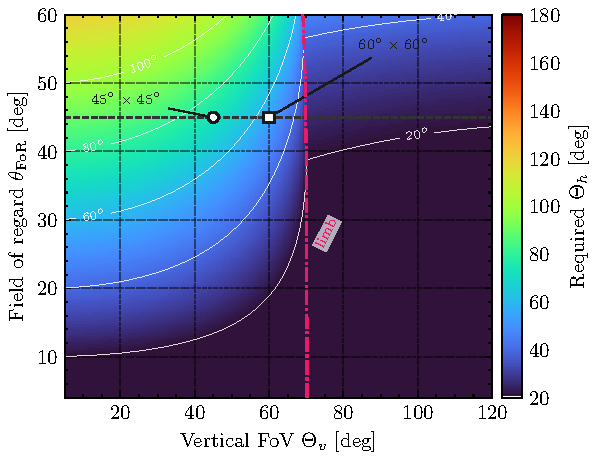
\includegraphics[width=\linewidth]{figures/horizontal_fov_design_map.pdf}
        \caption{Nadir FoR.}
        \label{fig:horizontal_fov_design_map_nadir}
    \end{subfigure}
    \hfill
    \begin{subfigure}[t]{0.49\linewidth}
        \centering
        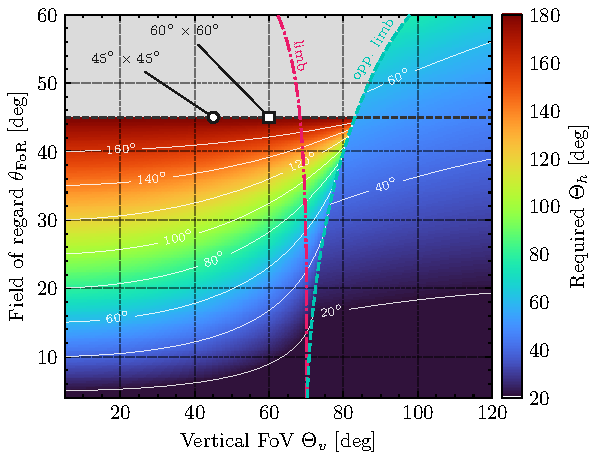
\includegraphics[width=\linewidth]{figures/rolled_body_fov_design_map.pdf}
        \caption{Rolled body, $\varphi=\theta_{\mathrm{FoR}}$.}
        \label{fig:horizontal_fov_design_map_rolled}
    \end{subfigure}
    \caption{Horizontal-FoV requirements induced by vertical FoV and field of regard at $h=\SI{400}{\kilo\metre}$. Heatmaps and contours show the minimum full horizontal FoV; the left panel uses the nadir-FoR requirement in~\eqref{eq:horizontal_fov_requirement}, while the right panel uses the rolled-body contact requirement in~\eqref{eq:rolled_body_horizontal_requirement}. The magenta dash-dotted curves mark where the limb first enters the corresponding detector/FoR geometry; the cyan dashed curve in the rolled panel marks when the opposite FoR edge reaches the detector at the horizon. In the rolled panel, the hatched region has no front-facing contact with both FoR edges inside the rectangular vertical detector band. The dashed line marks the $\pm$\ang{45} primary-imager field of regard used in this paper; markers show the representative \ang{45}$\times$\ang{45} and \ang{60}$\times$\ang{60} lookahead configurations.}
    \label{fig:horizontal_fov_design_map}
\end{figure}

\figref{fig:camera_fov_limit_boxes} visualizes these sizing constraints in common focal-plane coordinates.
The detector boxes are drawn on the same exterior $x/f,y/f$ basis in every panel, with the rolled-body row shown in the native rolled camera frame so that the detector centerline remains on the rolled boresight.

\begin{figure}[htbp]
    \centering
    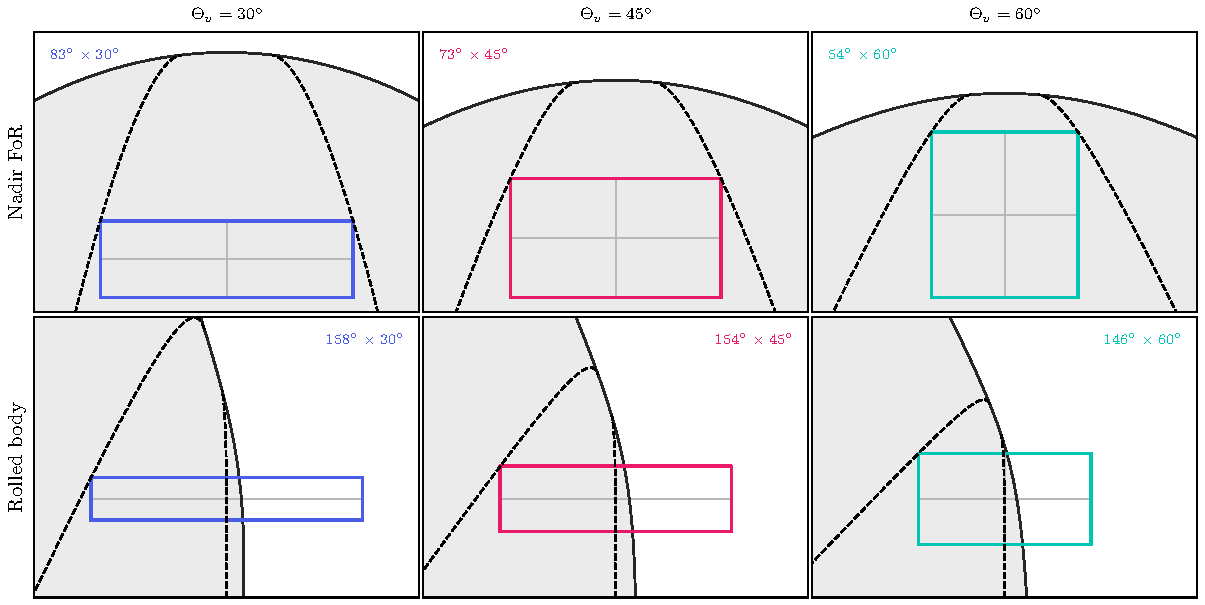
\includegraphics[width=\linewidth]{figures/camera_fov_limit_boxes.pdf}
    \caption{Common-focal camera views of detector boxes at the horizontal-FoV limits for vertical FoVs of \ang{30}, \ang{45}, and \ang{60}. Dashed curves are the field-of-regard envelopes, solid black curves are the horizon limb, shaded regions are Earth, and thin gray lines mark each detector's center axes. Columns vary the vertical FoV; the top row uses the nadir-FoR requirement at $\theta_{\mathrm{FoR}}=\ang{45}$, and the bottom row uses the native rolled-body camera frame at $\theta_{\mathrm{FoR}}=\ang{40}$ to show the near-\ang{180} body-fixed constraint.}
    \label{fig:camera_fov_limit_boxes}
\end{figure}

\paragraph{Instrument configurations.}
\tabref{tab:lookahead_cases} summarizes the two configurations analyzed here. The \emph{stationary} case satisfies the timing and nadir-FoR constraints without re-orientation; the \emph{agile} case sacrifices horizontal coverage and relies on spacecraft re-orientation.

\begin{table}[htbp]
\centering
\caption{Lookahead instrument configurations.}
\label{tab:lookahead_cases}
\begin{tabular}{@{}lccc@{}}
\toprule
\textbf{Case} & \textbf{Vertical FoV} & \textbf{Horizontal FoV} & \textbf{Boresight pitch} \\
\midrule
Stationary & \ang{60} & \ang{60} & \ang{30}   \\
Agile      & \ang{45} & \ang{45} & \ang{22.5} \\
\bottomrule
\end{tabular}
\end{table}

\subsection{Agility Limits}
\label{sec:agility_limits}

The same systems constraints define the limiting behavior of any dynamic-tasking policy.
With instantaneous slew, lookaheads can reveal every scheduled access before execution; if no gap can accommodate a round-trip maneuver, dynamic tasking collapses to the conventional schedule.

\begin{proposition}[Instant-slew omniscience]
\label{prop:omniscience}
Let $J_{\mathrm{omni}}$ denote the optimal MILP utility of~\eqref{eq:scheduling} under realized utilities $u_i = c_i \cdot X_i$ with cloud states $X_i$ revealed. In the limit $t_{\mathrm{slew}} \to 0$, any lookahead policy that observes each scheduled access before its imaging window achieves $J = J_{\mathrm{omni}}$.
\end{proposition}

The proof is given in Appendix~\ref{sec:appendix_proofs}.

\begin{corollary}[Monotonicity in agility]
\label{cor:monotone}
The set of feasible lookahead maneuvers is monotone non-increasing in $t_{\mathrm{slew}}$: any round-trip maneuver feasible at $t_{\mathrm{slew}}'$ is feasible at $t_{\mathrm{slew}} \leq t_{\mathrm{slew}}'$. Consequently, the optimal DT value $J^\star(t_{\mathrm{slew}})$ is non-increasing in $t_{\mathrm{slew}}$, ranging from $J_{\mathrm{omni}}$ at $t_{\mathrm{slew}} = 0$ down to $J_{\mathrm{conv}}$ once no gap admits any round-trip maneuver.
\end{corollary}

\noindent These limits bracket any dynamic-tasking policy without requiring additional simulation.

This system analysis reduces the onboard policy to one candidate lookahead action per schedule gap, searched over a discrete grid of feasible pitch angles.
The remaining question is how to value each candidate angle.

\section{Lookahead Decision Method}
\label{sec:method}

The decision rule is a local mean-field approximation to schedule repair inside a bounded lookahead window.
Its derivation uses four assumptions:
\begin{align}
&\textbf{(A1)}\quad \tau_{ij} \approx g \;\;\forall\,(i,j)\ \text{inside the local repair window}, && \text{constant effective spacing;} \notag\\
&\textbf{(A2)}\quad t_i \overset{\mathrm{i.i.d.}}{\sim} \mathcal{U}(T_1, T_2), && \text{exchangeable access times;} \notag\\
&\textbf{(A3)}\quad X_i \overset{\mathrm{i.i.d.}}{\sim} \mathrm{Bern}(p), && \text{i.i.d.\ cloud states;} \notag\\
&\textbf{(A4)}\quad c_i \approx \bar{c}, && \text{locally equal intrinsic utility.}
\label{eq:assumptions}
\end{align}
Assumption (A1) compresses detailed pairwise slews into the effective dead time used by the chain estimator.
Assumption (A2) is the symmetry exploited by the Poissonization step below: fixed-count uniform access times are equivalent to homogeneous Poisson arrivals conditioned on their count.
Assumptions (A3)--(A4) let the value calculation operate in expected clear-image equivalents; heterogeneous priorities can still enter through the schedule repair MILP after a lookahead is accepted.

\subsection{Two-Anchor Lookahead Value Model}
\label{sec:heuristic}

For a candidate pointing direction at pitch angle $\alpha$ (relative to the boresight rest angle $\alpha_0$), the camera projection determines which not-yet-observed accesses fall within the field of view at the lookahead imaging time.
Only visible accesses no earlier than the next scheduled image are scored, and we denote this set by $\mathcal{V}_\alpha$ with $N_{\mathrm{obs}}(\alpha)=|\mathcal{V}_\alpha|$.
For each schedule gap, the implementation fixes one comparison interval before scoring the pitch grid: $t_L$ is the previous scheduled image (or the planning-window start for the first gap), and $t_R$ is the first scheduled image after the largest feasible detector support over all candidate pitches.
Let
\begin{equation}
L_{\mathrm{anc}} = t_R - t_L
\label{eq:anchor_span}
\end{equation}
be the anchor-to-anchor interval.
All local times below are translated so that the left anchor is at $0$ and the right anchor is at $L_{\mathrm{anc}}$; this same anchor interval is used for every pitch in the gap.
The detector footprint need not span this whole interval.
For pitch $\alpha$, let
\begin{equation}
0 \leq \ell_\alpha < r_\alpha \leq L_{\mathrm{anc}},
\qquad
W_\alpha = r_\alpha-\ell_\alpha
\label{eq:detector_support}
\end{equation}
be the portion of the anchor interval covered by the lookahead detector after applying optimal timing, clipping the near edge at the next scheduled image, and clipping the far edge at the horizon.
Let $N_{\mathrm{sched}}$ be the number of scheduled imaging tasks in the open anchor interval $(t_L,t_R)$ and $N_{\mathrm{missed}}$ the number of scheduled tasks forfeited during the slew.
The net lookahead utility is
\begin{equation}
\widehat{\Delta J} = \underbrace{\hat{J}^+(\mathcal{V}_\alpha)}_{\text{advantage}} - \underbrace{\hat{J}^-(\mathcal{V}_\alpha)}_{\text{opportunity cost}}.
\label{eq:net_advantage}
\end{equation}

\paragraph{Opportunity cost.}
The cost side is local: each forfeited imaging task has expected clear utility $p \cdot \bar{c}$, giving
\begin{equation}
\hat{J}^- = p \cdot \bar{c} \cdot N_{\mathrm{missed}},
\label{eq:opp_cost}
\end{equation}
where $p = P(\text{clear})$ and $\bar{c}$ is the mean intrinsic utility.
The value-based policies below use the timing rule in \secref{sec:timing}, so $N_{\mathrm{missed}}=0$ during normal scoring; the term is retained for calibration windows and for non-optimal timing variants.

\paragraph{Poissonized chain model.}
The advantage side is harder because an observed clear access is valuable only if it can be inserted between the neighboring scheduled images without violating agility constraints.
The schedule anchors define the comparison interval, while the detector support defines where candidate accesses are actually revealed.
Within the clipped detector support, after thinning by the clear-sky prior, the effective clear-candidate density is
\begin{equation}
\lambda_{\mathrm{c}}(\alpha) = \frac{pN_{\mathrm{obs}}(\alpha)}{W_\alpha}.
\label{eq:clear_density}
\end{equation}
The stochastic step exploits the standard symmetry between fixed-count uniform samples and a conditioned Poisson process: conditional on seeing $N_{\mathrm{obs}}$ arrivals in the support interval, the unordered arrival times of a homogeneous Poisson process are i.i.d.\ uniform on that interval~\citep{feller_introduction_1991,david_order_2004}.
Thus the fixed set of visible candidate times can be modeled as a Poisson renewal process conditioned on its count; the onboard approximation then replaces the random clear subset by the unconditioned thinned process with rate $\lambda_{\mathrm{c}}$.
Compressing pairwise slew feasibility into an effective dead time $g$ turns the local repair problem into a one-dimensional packing problem.
With the left and right schedule anchors translated to $0$ and $L_{\mathrm{anc}}$, an insertable clear chain must satisfy
\begin{equation}
t_1 \geq g,\qquad
t_{i+1}-t_i \geq g,\qquad
L_{\mathrm{anc}}-t_k \geq g.
\label{eq:anchored_chain_constraints}
\end{equation}
The two scheduled anchors require one clearance interval at each boundary, but that requirement only removes detector support that lies too close to an anchor.
Define the boundary clearances
\begin{equation}
c_L(\alpha,g)=\max(0,\;g-\ell_\alpha),\qquad
c_R(\alpha,g)=\max(0,\;g-(L_{\mathrm{anc}}-r_\alpha)),
\label{eq:support_clearances}
\end{equation}
and the usable support length
\begin{equation}
U_\alpha(g)=W_\alpha-c_L(\alpha,g)-c_R(\alpha,g).
\label{eq:usable_support}
\end{equation}
After a chain member is accepted, the expected time until the next acceptable clear candidate is the deterministic clearance $g$ plus an exponential waiting time with mean $1/\lambda_{\mathrm{c}}$~\citep{feller_probability_1948,pyke_renewal_1958}.
Thus each additional insertable access consumes, on average,
\begin{equation}
\mathbb{E}[R] = g + \frac{1}{\lambda_{\mathrm{c}}},
\label{eq:renewal_spacing}
\end{equation}
where $R$ is the effective inter-registration spacing of the repaired chain.

For finite windows, the two-anchor chain probability keeps the boundary clearances explicit.
For detector support $[\ell_\alpha,r_\alpha]$ inside the anchor interval and Poisson clear-candidate rate $\lambda_{\mathrm{c}}$, the probability that at least $k$ internal points can be selected with all consecutive gaps at least $g$ is
\begin{equation}
G_\alpha(k;\,g) =
\frac{\gamma\!\big(k,\;\lambda_{\mathrm{c}}\bigl(U_\alpha(g) - (k{-}1)g\bigr)\big)}{\Gamma(k)},
\qquad U_\alpha(g) \geq (k{-}1)g,
\label{eq:chain_prob}
\end{equation}
with $G_\alpha(k;g)=0$ when $U_\alpha(g) < (k{-}1)g$.
The corresponding expected number of insertable internal points is
\begin{equation}
\widehat{K}_{2a}(\alpha,g)
=
\sum_{k\geq 1}
G_\alpha(k;\,g).
\label{eq:chain_expectation}
\end{equation}
When the detector support spans the full anchor interval, $\ell_\alpha=0$ and $r_\alpha=L_{\mathrm{anc}}$, so $c_L=c_R=g$ and~\eqref{eq:chain_prob} reduces to the usual two-boundary form with residual length $L_{\mathrm{anc}}-(k{+}1)g$.
This gives the finite-window advantage score
\begin{equation}
\hat{J}^+_{2a}
=
\bar{c}\,\widehat{K}_{2a}(\alpha,g),
\label{eq:renewal_advantage}
\end{equation}
where the subscript $2a$ denotes the two scheduled anchors.
The exact onboard gate could evaluate $\widehat{K}_{2a}(\alpha,g_{\mathrm{phys}})$ directly; the summation is finite, monotone in $g$, and cheap for the short local windows considered here.

\paragraph{Break-even approximation.}
For a lightweight threshold, we approximate the finite-window chain by its long-run renewal rate on the same usable detector support:
\begin{equation}
\widehat{K}_{b}(\alpha,g)
\;\approx\;
\frac{U_\alpha(g)}{g + 1/\lambda_{\mathrm{c}}(\alpha)}
\;=\;
\frac{\lambda_{\mathrm{c}}(\alpha)U_\alpha(g)}
{1 + \lambda_{\mathrm{c}}(\alpha) g}.
\label{eq:chain_rational_approx}
\end{equation}
This approximation replaces the finite-window chain distribution by its average packing rate.
It has the required behavior for onboard gating: value increases with observed candidate density and decreases monotonically with dead time.
The finite two-anchor form is the higher-fidelity value estimator; $\widehat{K}_{b}$ is the algebraic surrogate that yields a monotone break-even spacing.
Appendix~\ref{sec:appendix_renewal} derives~\eqref{eq:chain_prob} and discusses the residual bias.

\begin{figure}[htbp]
    \centering
    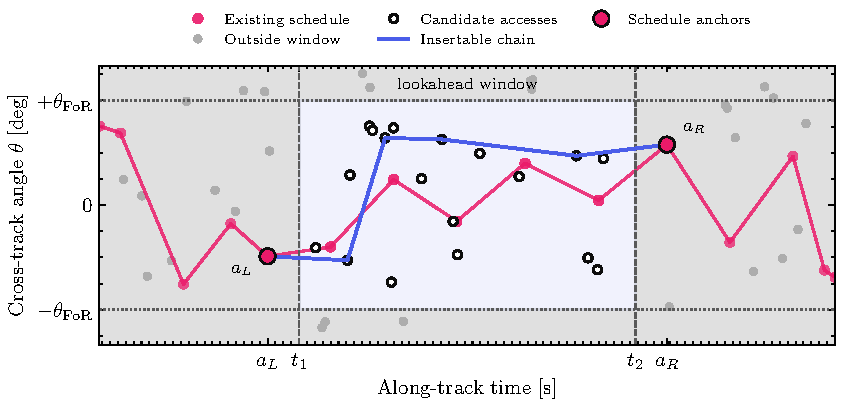
\includegraphics[width=.8\linewidth]{figures/chain_abstraction.pdf}
    \caption{Anchor-bounded lookahead window used by the two-anchor value model. The two scheduled anchors bound the local repair subgraph; gray regions are outside the actionable lookahead window. The model asks whether the expected utility from insertable candidate accesses inside the window exceeds the local replacement burden.}
    \label{fig:chain_abstraction}
\end{figure}

Now write the net advantage in units of average task utility:
\begin{equation}
\frac{\widehat{\Delta J}_{2a}}{\bar{c}}
=
\widehat{K}_{2a}(\alpha,g)
-
\left(p\,N_{\mathrm{sched}} + \frac{\hat{J}^-}{\bar{c}}\right).
\label{eq:normalised_advantage}
\end{equation}
Define the second term as
\begin{equation}
B \;=\; p\,N_{\mathrm{sched}} + \frac{\hat{J}^-}{\bar{c}},
\label{eq:break_even_baseline}
\end{equation}
the number of clear captures that the lookahead must beat: the expected clear captures already present in the local schedule plus any expected opportunity cost from displaced tasks.
Physically, $B$ is the local replacement burden, measured in equivalent unit-clear images.
The first term, $pN_{\mathrm{sched}}$, is the expected number of already-scheduled images in the observation window that the repaired schedule must at least preserve in expectation.
The second term, $\hat{J}^-/\bar{c}$, converts any maneuver-induced loss of scheduled utility into the same units.
Thus $B$ is not a cloud or geometry parameter by itself; it is the number of clear-image equivalents the lookahead must produce before it creates net schedule value.
For pitch search, $B$ is fixed once per schedule gap using the common anchor interval above, while $\mathcal{V}_\alpha$, $W_\alpha$, $\ell_\alpha$, and $r_\alpha$ remain pitch-dependent.
The finite-window gate is therefore $\widehat{K}_{2a}(\alpha,g_{\mathrm{phys}})>B$.
For an onboard engineering threshold, set $\widehat{K}_{b}(\alpha,g_{\mathrm{break}})=B$ using the rational approximation in~\eqref{eq:chain_rational_approx}.
Equivalently,
\begin{equation}
g_{\mathrm{break}}(\alpha)
=
\sup\left\{
g \geq 0:
\frac{\lambda_{\mathrm{c}}(\alpha)U_\alpha(g)}
{1+\lambda_{\mathrm{c}}(\alpha)g}
> B
\right\}.
\label{eq:g_break_alpha}
\end{equation}
If $\lambda_{\mathrm{c}}(\alpha)U_\alpha(0) \leq B$, even a zero-dead-time chain cannot beat the local baseline in this approximation, so the candidate window has no positive break-even spacing.
When the detector support spans the full anchor interval, $\ell_\alpha=0$ and $r_\alpha=L_{\mathrm{anc}}$, \eqref{eq:g_break_alpha} reduces to the closed form
\begin{equation}
g_{\mathrm{break}}
\;\approx\;
\frac{L_{\mathrm{anc}}\left(pN_{\mathrm{obs}} - B\right)}
{pN_{\mathrm{obs}}\left(2+B\right)},
\qquad pN_{\mathrm{obs}} > B.
\label{eq:g_break_full_support}
\end{equation}
Since the packing estimate decreases monotonically with $g$, the lookahead gate can be interpreted as
\begin{equation}
\widehat{\Delta J} > 0
\quad\Longleftrightarrow\quad
g_{\mathrm{phys}} < g_{\mathrm{break}},
\label{eq:break_even_gate}
\end{equation}
up to the approximation in~\eqref{eq:chain_rational_approx}.

This is the key interpretation: $g_{\mathrm{break}}$ is not a replacement for the spacecraft slew time.
It is the maximum effective dead time that the current observation window can tolerate before the expected value of looking falls to zero.
In the common case where opportunity cost is zeroed by optimal timing and the baseline term is dominated by $pN_{\mathrm{sched}}$, this threshold scales with the usable detector support per replacement burden.

The pointing optimization belongs inside this threshold.
For each feasible pitch angle $\alpha$, the camera projection and timing rule induce a different observed-access set, detector support $[\ell_\alpha,r_\alpha]$, and boundary clearances inside the fixed gap-level baseline.
The practical decision variable is therefore the break-even margin
\begin{equation}
M(\alpha)
= g_{\mathrm{break}}(\alpha) - g_{\mathrm{phys}}(\alpha),
\qquad
\alpha^\dagger = \arg\max_{\alpha \in \mathcal{G}_{\alpha}^{\mathrm{feas}}} M(\alpha),
\label{eq:break_even_margin}
\end{equation}
and the lookahead is accepted only when $M(\alpha^\dagger)>0$.
The two-anchor policy reported in the experiments uses the same support and baseline construction but maximizes $\widehat{K}_{2a}(\alpha,g_{\mathrm{phys}})-B$ directly instead of the break-even margin.
For the body-fixed configuration, $g_{\mathrm{phys}}(\alpha)=t_{\mathrm{slew}}(\theta_{\mathrm{FoR}})$ in the chain estimator because the repaired imaging sequence must still tolerate worst-case cross-track slews across the primary imager's field of regard.
The pitch angle $\alpha$ affects the margin through $N_{\mathrm{obs}}(\alpha)$, $W_\alpha$, $\ell_\alpha$, $r_\alpha$, and maneuver feasibility; architectures with angle-dependent imaging dead time can instead substitute their physical $g_{\mathrm{phys}}(\alpha)$ directly into~\eqref{eq:break_even_margin}.

\subsection{Lookahead Sensing Policy: Timing and Pitch}
\label{sec:lookahead_policy}

The value model scores a candidate observation window.
The resulting sensing policy maps the onboard state at a schedule gap to either a lookahead action or the no-look action; if it looks, it must choose when the lookahead occurs and which pitch angle defines the observation window.
Timing is analytic, leaving a one-dimensional pitch search.

\paragraph{Optimal lookahead timing.}
\label{sec:timing}
Let a \emph{schedule gap} $[t_{\mathrm{prev}} + t_s,\; t_{\mathrm{next}}]$ be a maximal idle interval between consecutive imaging tasks.
Timing trades two opposing effects: a later observation sees further into the future and reveals more clear candidates (growing $\hat{J}^+$), but if the round-trip maneuver extends past $t_{\mathrm{next}}$ it begins to displace the next scheduled task (growing $\hat{J}^-$).
The best of both worlds is the latest time at which the maneuver still ends before $t_{\mathrm{next}}$:
\begin{equation}
t^\star(\alpha) = t_{\mathrm{next}} - t_{\mathrm{man}}(\alpha),
\label{eq:optimal_timing}
\end{equation}
where $t_{\mathrm{man}}(\alpha) = 2(t_{\mathrm{slew}}(\alpha - \alpha_0) - t_s)$ is the round-trip maneuver time for pitch angle $\alpha$ and the \emph{actionable} observation window has length
\begin{equation}
L_{\mathrm{act}}(t) = t + t_{\mathrm{horizon}} - t_{\mathrm{next}}.
\label{eq:actionable_window}
\end{equation}

\begin{proposition}[Optimal Lookahead Timing]
\label{prop:timing}
Within a schedule gap, $t = t^\star(\alpha)$ maximizes the net advantage $\widehat{\Delta J}$ up to a bounded perturbation of size $p\bar{c}$, at which point $\hat{J}^- = 0$ and the value gate is evaluated on the clipped detector support inside the fixed gap-level anchor interval.
\end{proposition}

A lookahead at angle $\alpha$ is feasible only if the gap accommodates the maneuver: $t_{\mathrm{next}} - t_{\mathrm{prev}} - t_s \geq t_{\mathrm{man}}(\alpha)$.
The formal proof, including the bounded-perturbation bookkeeping at scheduled-access entries, is given in Appendix~\ref{sec:appendix_proofs}.

\paragraph{Break-even pointing search.}
\label{sec:joint_opt}
Since $t^\star$ depends on $\alpha$, pitch trades access count against maneuver time: steeper pitch observes more accesses but shrinks the actionable window.
The break-even rule evaluates~\eqref{eq:g_break_alpha} over a discrete grid of feasible angles and accepts a lookahead when the best margin in~\eqref{eq:break_even_margin} is positive.
The pitch dependence enters through both the visible-access count and the clipped detector support, while the replacement baseline is held fixed across the pitch grid for that schedule gap.
The implemented policy takes the sensing action $\alpha^\dagger$ from~\eqref{eq:break_even_margin} if $M(\alpha^\dagger)>0$, and takes the no-look action otherwise.

\subsection{Schedule Repair}
\label{sec:schedule_repair}

Once the policy chooses a positive-value lookahead, the spacecraft executes the maneuver, observes the visible accesses, and repairs only the affected schedule segment.
The repair uses receding-horizon re-optimization~\cite{boerkoel_efficient_2021}, treating the lookahead as a schedule-level action gated by the heuristic~\cite{nag_autonomous_2019, augenstein_optimal_2016}.
The spacecraft maintains both a pre-optimized schedule and a priority queue of alternate accesses.
The repair operates on a local subgraph bounded by the nearest scheduled tasks before and after the observation window, which are forced into the MILP to anchor the repaired segment back to the original schedule.
Observed-cloudy accesses are removed from the candidate set; observed-clear and unobserved accesses remain available, with unobserved accesses retaining their prior expected utility $p \cdot c_i$.
The repaired segment is spliced back into the full schedule, and the spacecraft advances to the next imaging block.

Algorithm~\ref{alg:dt_loop} summarizes the full onboard control loop.

\begin{algorithm}[htbp]
\caption{Dynamic tasking control loop}
\label{alg:dt_loop}
\begin{algorithmic}[1]
\Require initial schedule $\boldsymbol{\sigma}_0$, alternates queue $\mathcal{A}_{\text{alt}}$, angle grid $\mathcal{G}_\alpha$, cloud prior $p$
\State $\boldsymbol{\sigma} \gets \boldsymbol{\sigma}_0$
\For{each schedule gap $[t_{\mathrm{prev}}+t_s,\, t_{\mathrm{next}}]$ in $\boldsymbol{\sigma}$}
    \State $\alpha^\dagger \gets \arg\max_{\alpha \in \mathcal{G}_\alpha^{\mathrm{feas}}} M(\alpha)$ \Comment{break-even margin in~\eqref{eq:break_even_margin}}
    \If{$M(\alpha^\dagger) > 0$ \textbf{and} $t_{\mathrm{next}} - t_{\mathrm{prev}} - t_s \geq t_{\mathrm{man}}(\alpha^\dagger)$}
        \State at $t^\star(\alpha^\dagger) = t_{\mathrm{next}} - t_{\mathrm{man}}(\alpha^\dagger)$: slew to $\alpha^\dagger$, observe, slew back \Comment{Prop.~\ref{prop:timing}}
        \State update $\{X_i\}$ for accesses in the observed window
        \State $\boldsymbol{\sigma} \gets \textsc{MILP-Repair}(\boldsymbol{\sigma},\, \mathcal{A}_{\text{alt}},\, \text{bounding accesses})$
    \EndIf
    \State execute scheduled imaging in $[t_{\mathrm{prev}}, t_{\mathrm{next}}]$
\EndFor
\end{algorithmic}
\end{algorithm}
